\documentclass[UTF8,a4paper,11pt]{ctexart}

\usepackage{amsmath}
\usepackage{booktabs}
\usepackage{caption}
\usepackage{float}
\usepackage{geometry}
\usepackage{graphicx}
\usepackage{hyperref}
\usepackage{longtable}
\usepackage{tabularx}
\usepackage{url}
\usepackage{xcolor}

\geometry{left=2.5cm,right=2.5cm,top=2.6cm,bottom=2.6cm}
\graphicspath{{figures/}}
\hypersetup{
  colorlinks=true,
  linkcolor=blue,
  urlcolor=blue,
  citecolor=blue
}

\newcommand{\todo}[1]{\textcolor{red}{【待补充：#1】}}
\newcommand{\metric}[1]{\textbf{#1}}

\title{深度学习与空间智能 Homework 2 实验报告}
\author{
  \todo{姓名1 / 学号1 / 分工}\\
  \todo{姓名2 / 学号2 / 分工}
}
\date{2026 年 5 月}

\begin{document}

\maketitle

\begin{center}
\begin{tabular}{ll}
\toprule
代码仓库 & \url{https://github.com/zj-yao/Homework_2}\\
模型权重 & \todo{填写百度云、Google Drive 或其他网盘链接}\\
运行环境 & NVIDIA GeForce RTX 3060 12GB, PyTorch 2.5.1 + CUDA 12.1\\
\bottomrule
\end{tabular}
\end{center}

\begin{abstract}
本次作业完成了三个深度学习实验：在 Oxford 102 Category Flower Dataset 上微调 ImageNet 预训练 CNN 进行花卉分类；在 Road Vehicle Images Dataset 上微调 YOLOv8，并在自录道路视频上完成多目标跟踪、遮挡分析和越线计数；从零实现 U-Net，在 Stanford Background Dataset 上比较 Cross-Entropy Loss、Dice Loss 与二者组合对语义分割 mIoU 的影响。实验结果表明，ImageNet 预训练显著提升小样本花卉分类效果；YOLOv8s 相比 YOLOv8n 在车辆检测上获得更高 mAP；在语义分割中 CE + Dice 组合损失取得最高验证 mIoU。
\end{abstract}

\section{实验概述}

作业 PDF 的第一项标题中出现了“宠物识别”的表述，但正文明确要求使用 102 Category Flower Dataset。因此本文按正文要求完成花卉分类实验。三个任务的主要目标如下：

\begin{enumerate}
  \item 花卉分类：使用 ResNet-18/ResNet-34 迁移学习，比较预训练、随机初始化、学习率变化和注意力模块。
  \item 车辆检测与跟踪：使用 YOLOv8 微调车辆检测器，并在 10--30 秒道路视频上展示 Tracking ID、遮挡片段和越线计数。
  \item 语义分割：手写 U-Net，不使用预训练权重，比较 CE、Dice、CE + Dice 三种损失函数。
\end{enumerate}

所有实验使用固定随机种子 42。训练过程保存配置、历史 CSV、最优 checkpoint 和评估结果；训练可视化图由本地日志与 CSV 文件导出生成。

\section{实验环境与数据集}

\subsection{实验环境}

实验在 conda 环境 \path{dl_hw2} 中运行。主要软件与硬件如下：

\begin{table}[H]
\centering
\caption{实验环境}
\begin{tabular}{ll}
\toprule
项目 & 配置 \\
\midrule
GPU & NVIDIA GeForce RTX 3060, 12GB VRAM \\
Python & 3.10.20 \\
PyTorch & 2.5.1 + CUDA 12.1 \\
Torchvision & 0.20.1 + CUDA 12.1 \\
Ultralytics & 8.4.41 \\
OpenCV & 4.13.0 \\
日志工具 & SwanLab offline logging \\
\bottomrule
\end{tabular}
\end{table}

\subsection{数据集划分}

\begin{table}[H]
\centering
\caption{数据集与划分}
\begin{tabularx}{\textwidth}{lXl}
\toprule
任务 & 数据集 & 划分 \\
\midrule
分类 & 102 Category Flower Dataset & 官方划分：train 1020、val 1020、test 6149，类别数 102 \\
检测 & Road Vehicle Images Dataset & YOLO 格式：train 2704、valid 300，类别数 21 \\
分割 & Stanford Background Dataset & train 572、val 143，类别数 8 \\
\bottomrule
\end{tabularx}
\end{table}

分类任务使用 \path{torchvision.datasets.Flowers102} 的官方划分。检测任务使用 Kaggle Road Vehicle 数据集中的 YOLO 标注目录 \path{trafic_data}。分割任务使用 Stanford Background 的图像与 \path{labels/*.regions.txt} 标签，并转换为整数类别 mask。

\section{任务一：花卉分类}

\subsection{方法}

分类模型以 ResNet-18 为主要基线，并补充 ResNet-34 增强实验。对于 ImageNet 预训练模型，最后的全连接层被替换为 102 类输出层。优化器使用 AdamW，并设置参数组：backbone 使用较小学习率，分类头使用较大学习率。输入图像缩放到 $224 \times 224$；训练增强包括 RandomResizedCrop、RandomHorizontalFlip 和 ImageNet 均值方差归一化。

注意力实验使用 SE block。其核心思想是先通过全局平均池化得到通道描述，再用两层 $1 \times 1$ 卷积学习通道权重，最后将权重乘回特征图。实验中将 ResNet-18 的 BasicBlock 替换为带 SE 的 BasicBlock。

\subsection{训练设置}

\begin{table}[H]
\centering
\caption{分类任务主要训练设置}
\begin{tabular}{ll}
\toprule
项目 & 设置 \\
\midrule
输入尺寸 & $224 \times 224$ \\
Batch size & 32 \\
Optimizer & AdamW, weight decay $1\times10^{-4}$ \\
Loss & Cross-Entropy Loss \\
Baseline LR & backbone $1\times10^{-4}$, head $1\times10^{-3}$ \\
Low LR & backbone $5\times10^{-5}$, head $5\times10^{-4}$ \\
High LR & backbone $2\times10^{-4}$, head $2\times10^{-3}$ \\
Metric & Validation accuracy, test accuracy \\
\bottomrule
\end{tabular}
\end{table}

\subsection{结果}

\begin{table}[H]
\centering
\caption{花卉分类实验结果}
\small
\begin{tabular}{lcccccc}
\toprule
实验 & 预训练 & 注意力 & Epoch & Backbone LR & Head LR & Test Acc \\
\midrule
ResNet18 baseline & 是 & 无 & 30 & $1\times10^{-4}$ & $1\times10^{-3}$ & 0.8853 \\
ResNet18 baseline & 是 & 无 & 15 & $1\times10^{-4}$ & $1\times10^{-3}$ & 0.8785 \\
ResNet18 low LR & 是 & 无 & 15 & $5\times10^{-5}$ & $5\times10^{-4}$ & 0.8666 \\
ResNet18 high LR & 是 & 无 & 15 & $2\times10^{-4}$ & $2\times10^{-3}$ & 0.8862 \\
ResNet18 random init & 否 & 无 & 30 & $1\times10^{-4}$ & $1\times10^{-3}$ & 0.3627 \\
ResNet18 + SE & 是 & SE & 30 & $1\times10^{-4}$ & $1\times10^{-3}$ & 0.8580 \\
ResNet34 enhanced & 是 & 无 & 60 & $1\times10^{-4}$ & $1\times10^{-3}$ & \metric{0.8863} \\
\bottomrule
\end{tabular}
\end{table}

\begin{figure}[H]
\centering
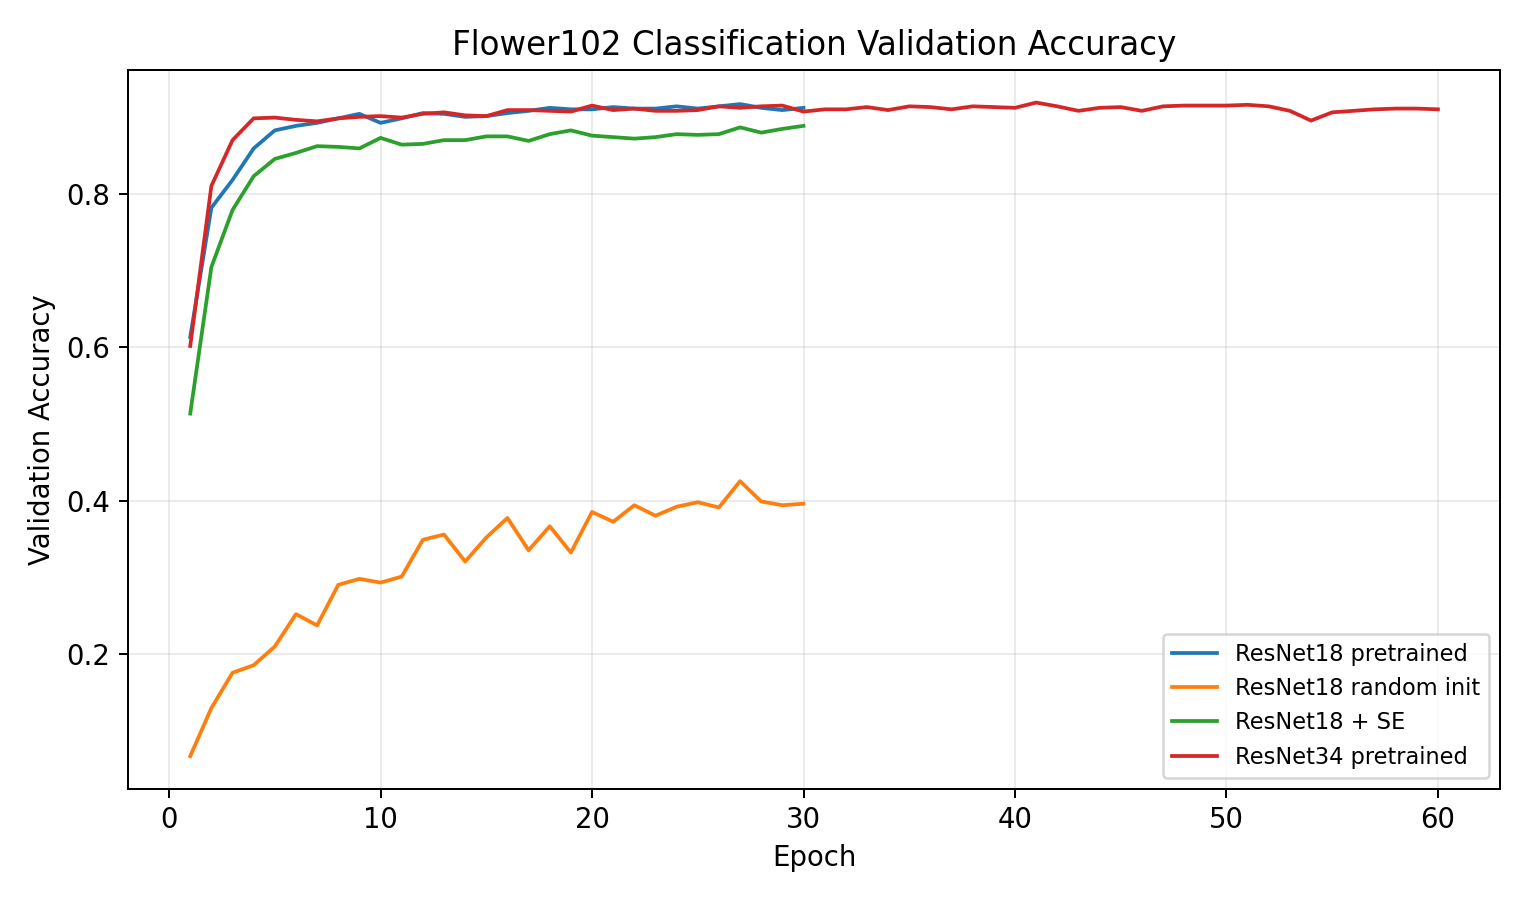
\includegraphics[width=0.82\textwidth]{classification_val_accuracy.png}
\caption{分类任务验证集 Accuracy 曲线}
\end{figure}

\begin{figure}[H]
\centering
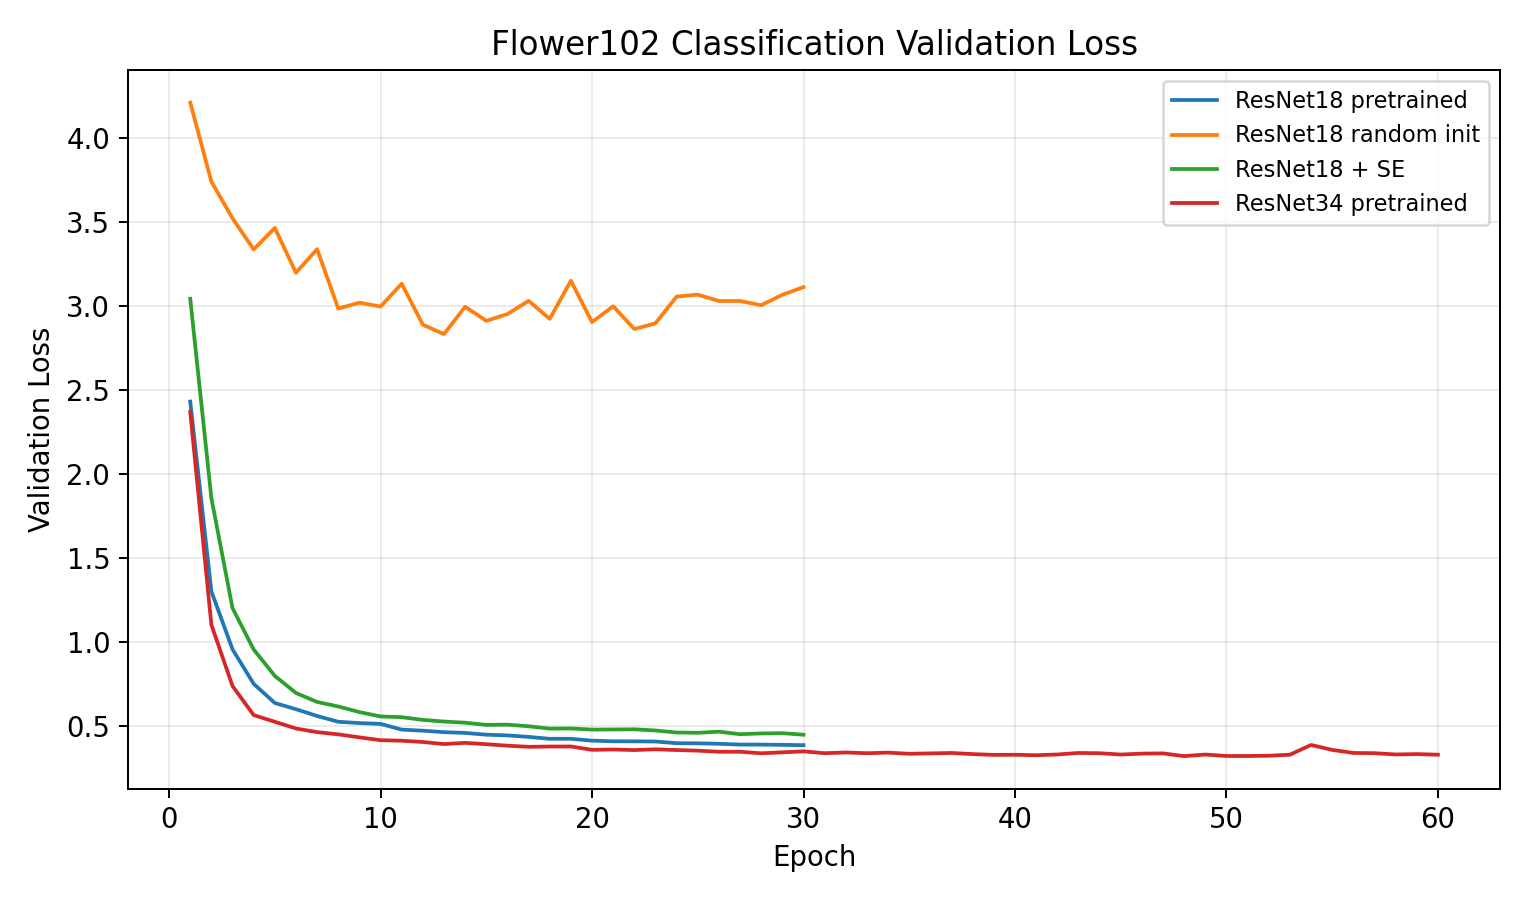
\includegraphics[width=0.82\textwidth]{classification_val_loss.png}
\caption{分类任务验证集 Loss 曲线}
\end{figure}

从结果可以看到，ImageNet 预训练对 Flower102 这种每类训练样本较少的数据集非常重要。随机初始化的 ResNet-18 在 30 个 epoch 后 test accuracy 只有 0.3627，而预训练 ResNet-18 达到 0.8853。学习率对最终效果也有影响，15 epoch 的 high LR 设置与 30 epoch baseline 和 60 epoch ResNet-34 基本持平。SE block 在本实验中没有提升结果，说明注意力模块并非必然改善性能；在训练轮数、学习率、数据增强没有重新调优时，额外模块可能带来优化难度或轻微过拟合。

\section{任务二：车辆检测、跟踪与计数}

\subsection{检测模型与训练设置}

检测任务使用 Ultralytics YOLOv8。数据集配置为 21 个车辆与交通相关类别，训练图像 2704 张，验证图像 300 张。实验先训练 YOLOv8n 作为轻量基线，再训练 YOLOv8s 作为增强模型。两者均使用 $640 \times 640$ 输入、batch size 8、AMP 混合精度和固定随机种子 42。

\begin{table}[H]
\centering
\caption{车辆检测实验结果}
\begin{tabular}{lccccc}
\toprule
模型 & Epoch & Precision & Recall & mAP50 & mAP50-95 \\
\midrule
YOLOv8n & 50 & 0.5952 & 0.3833 & 0.4315 & 0.2648 \\
YOLOv8s & 100 & \metric{0.7359} & \metric{0.4597} & \metric{0.5220} & \metric{0.3108} \\
\bottomrule
\end{tabular}
\end{table}

\begin{figure}[H]
\centering
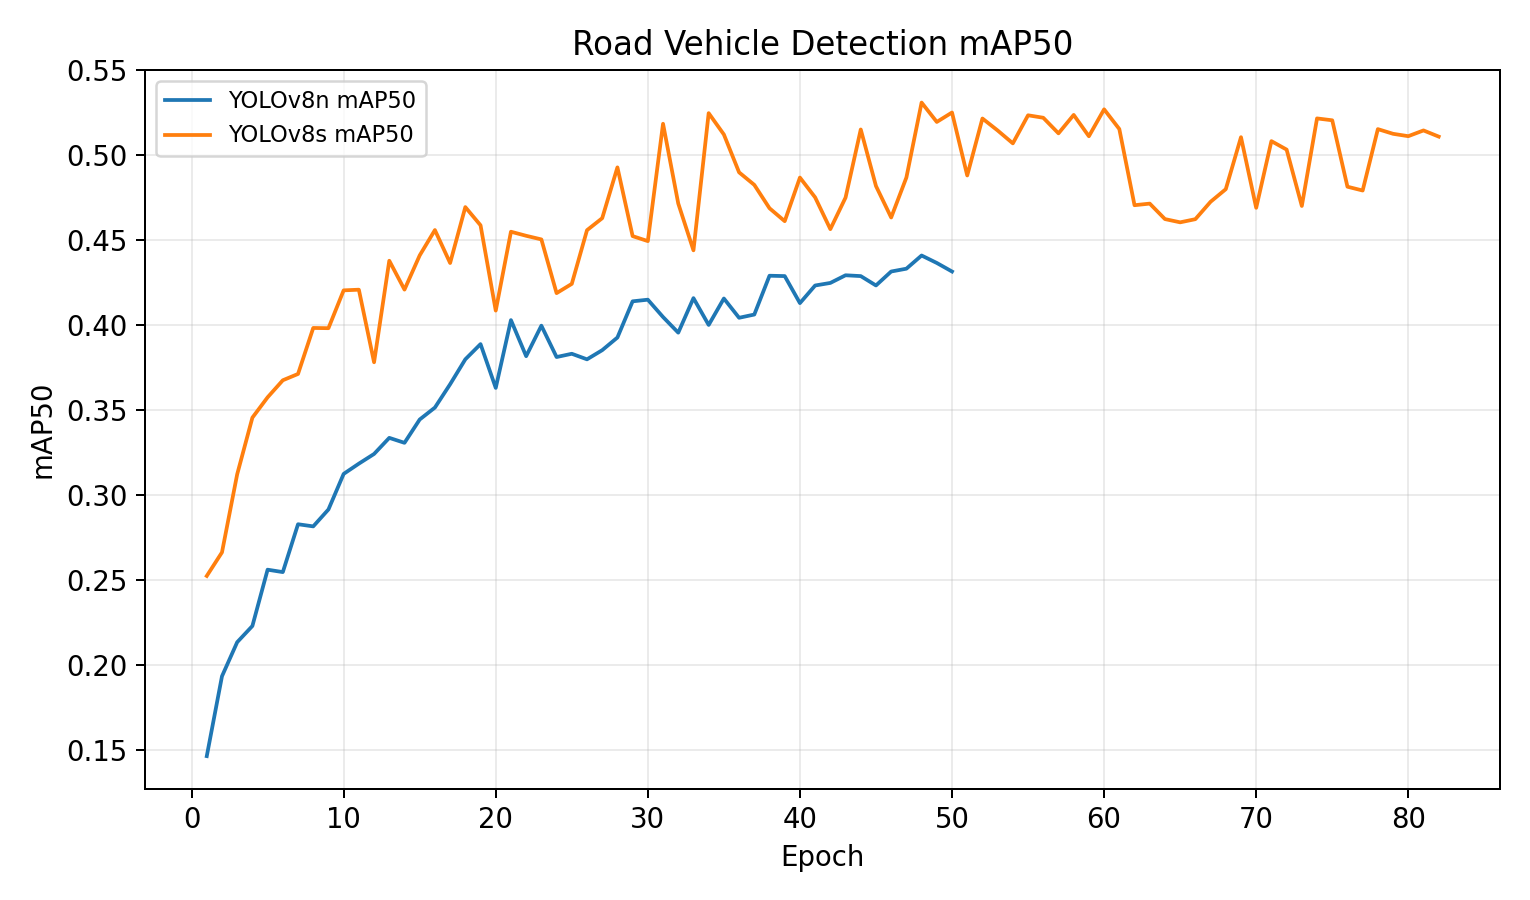
\includegraphics[width=0.82\textwidth]{detection_map50.png}
\caption{车辆检测 mAP50 曲线}
\end{figure}

\begin{figure}[H]
\centering
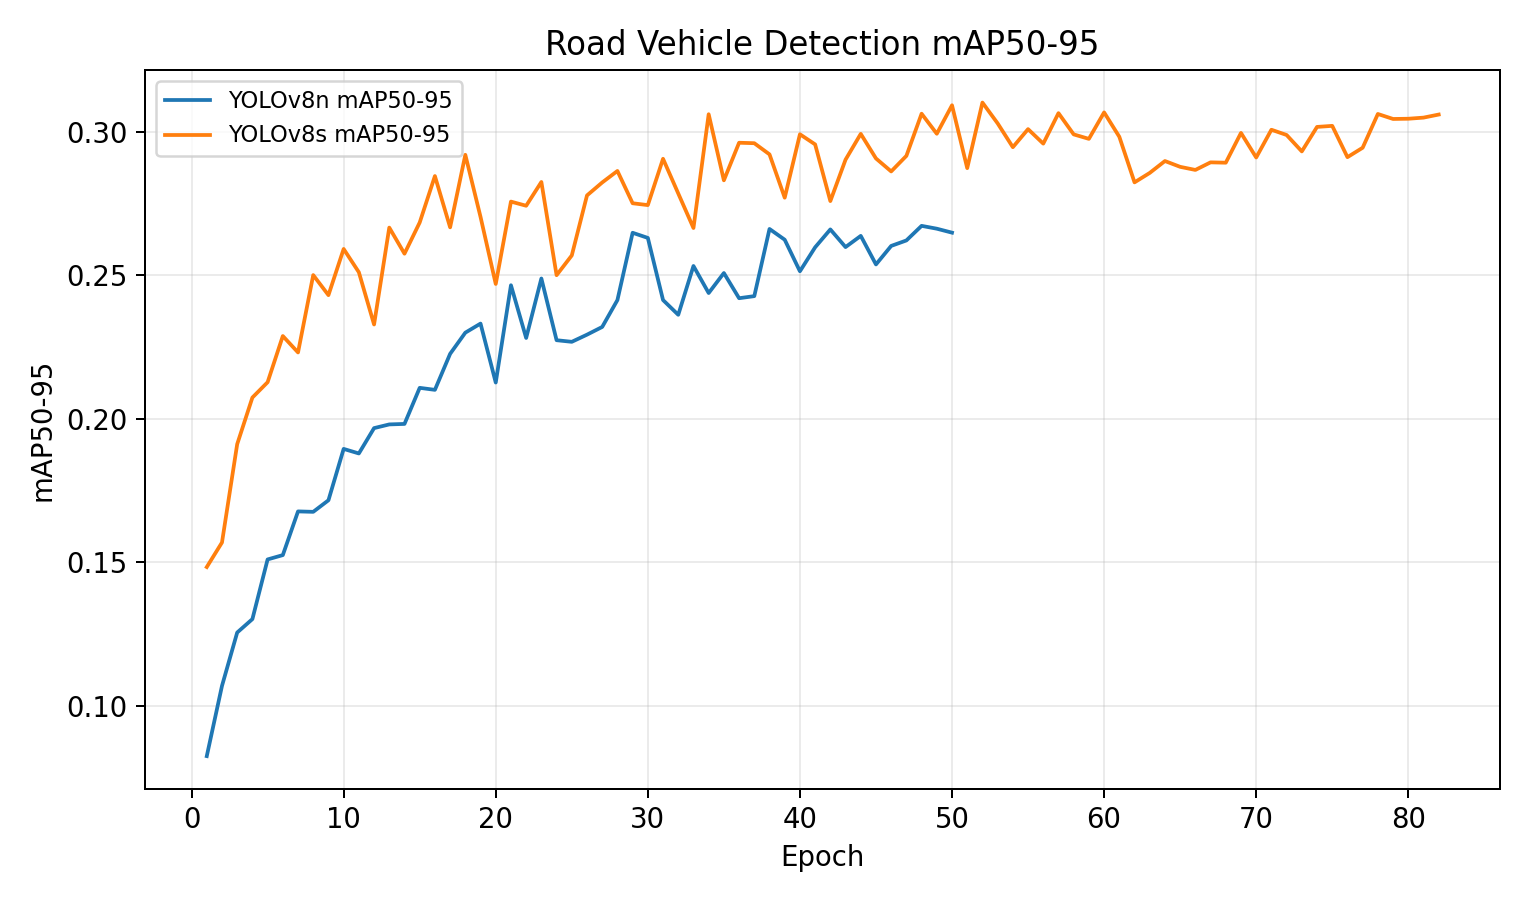
\includegraphics[width=0.82\textwidth]{detection_map50_95.png}
\caption{车辆检测 mAP50-95 曲线}
\end{figure}

\begin{figure}[H]
\centering
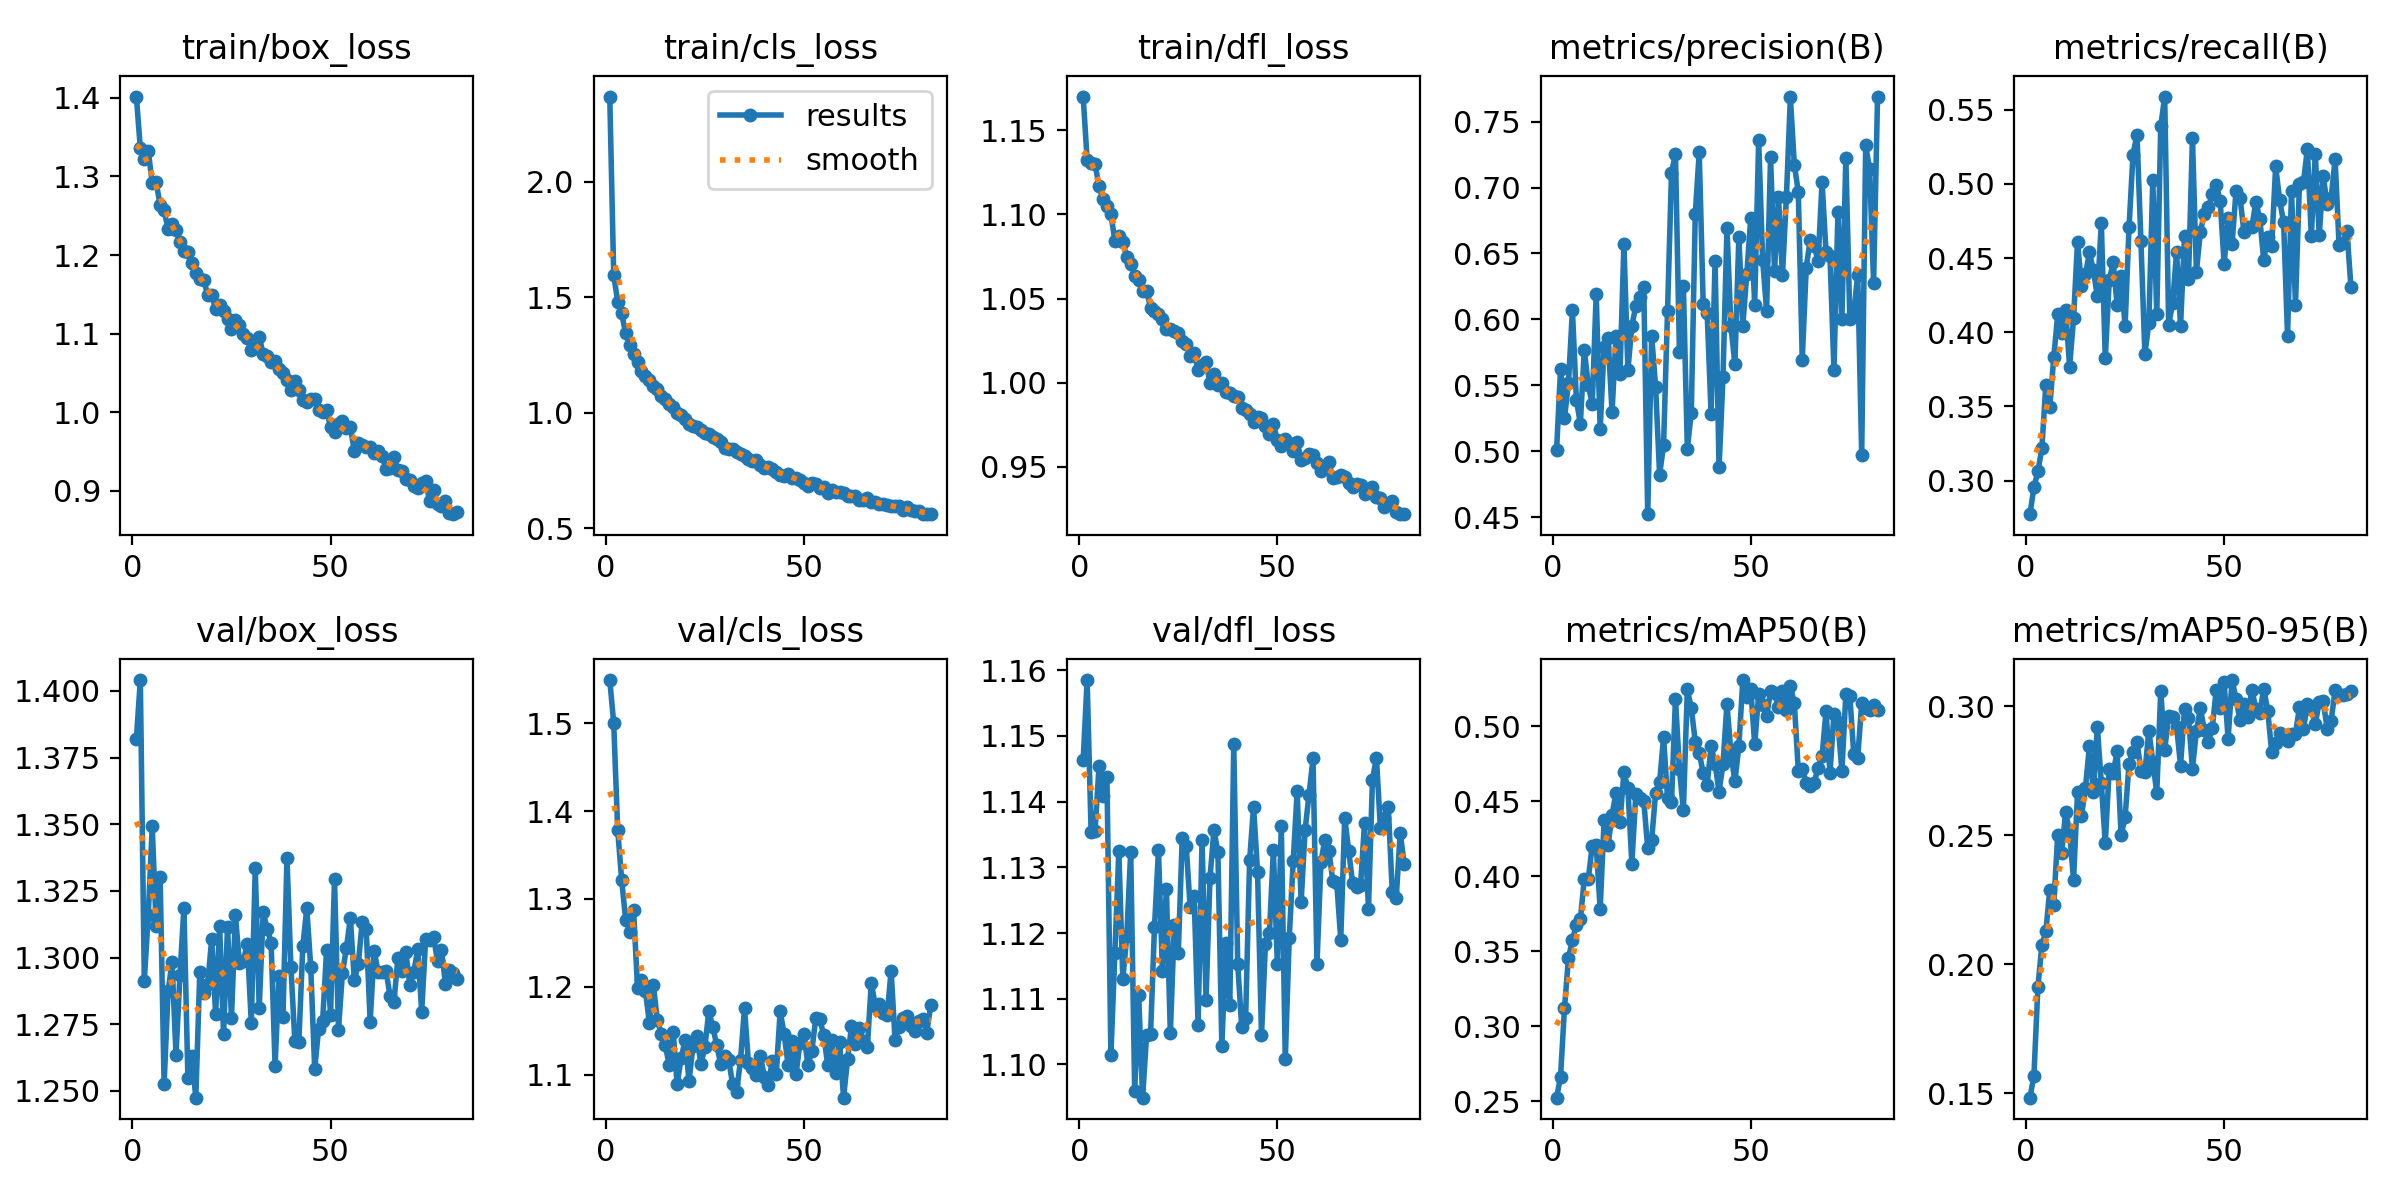
\includegraphics[width=0.92\textwidth]{yolov8s_results.png}
\caption{YOLOv8s 训练过程可视化}
\end{figure}

YOLOv8s 相比 YOLOv8n 在 precision、recall 和 mAP 上均有提升。由于 YOLOv8s 的模型容量更大、训练 epoch 更多，它更适合作为后续视频跟踪的检测器。

\subsection{视频跟踪与越线计数}

测试视频为自行录制道路车辆视频，文件为 \path{data/videos/campus_road_01.mp4}，时长约 19.53 秒，帧率 30 FPS，分辨率 $1280 \times 720$。跟踪模型使用训练后的 YOLOv8s 权重，并调用 ByteTrack 进行关联。输出视频为：

\begin{center}
\path{outputs/detection_tracking/tracked_video/campus_road_01_yolov8s_tracked_counted.mp4}
\end{center}

程序在每一帧绘制检测框、类别、置信度和 Tracking ID。越线计数使用一条竖直虚拟线，从 $(640,180)$ 到 $(640,720)$。对每个 Tracking ID 保存上一帧和当前帧的检测框中心点；当中心轨迹跨过计数线时计数一次，并将该 ID 加入已计数集合，避免重复计数。最终计数结果为 5，对应 crossed IDs 为 1、24、26、67、90。

\begin{figure}[H]
\centering
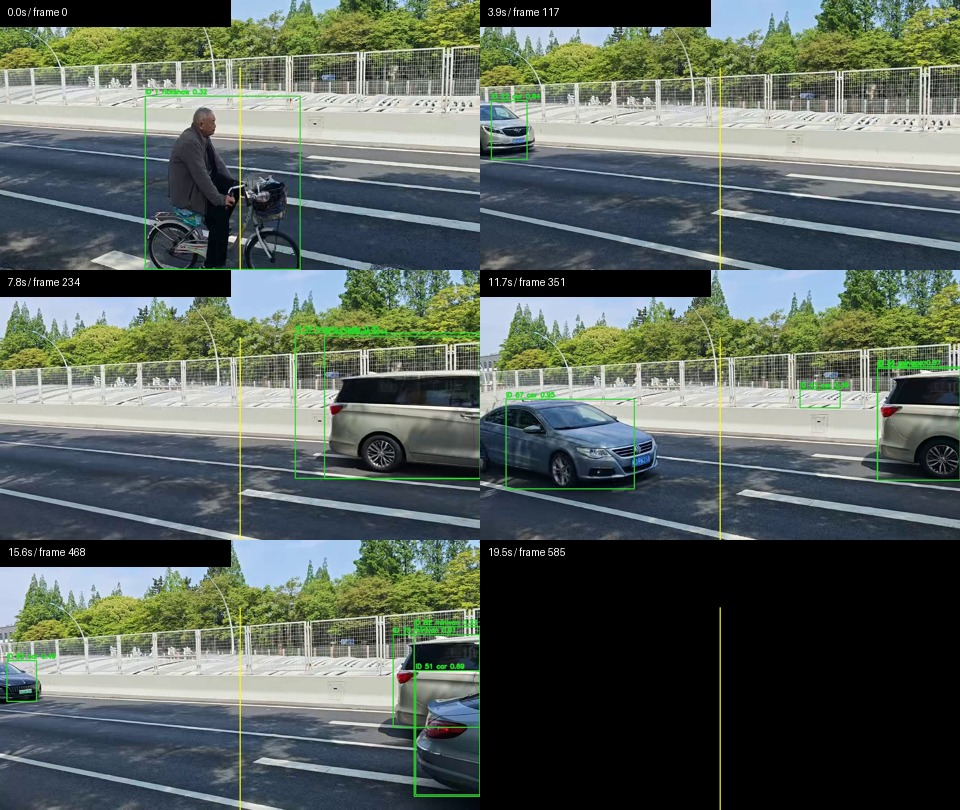
\includegraphics[width=0.92\textwidth]{tracking_contact_sheet.jpg}
\caption{视频跟踪与越线计数示例帧}
\end{figure}

\subsection{遮挡与 ID 分析}

遮挡分析选取视频第 536--539 帧，对应约 17.87--17.97 秒。该片段中，前景白色车辆经过画面下方，同时右侧车辆仍部分可见。连续帧中可见跟踪器基本保持 ID，没有观察到明显 ID switch。

\begin{figure}[H]
\centering
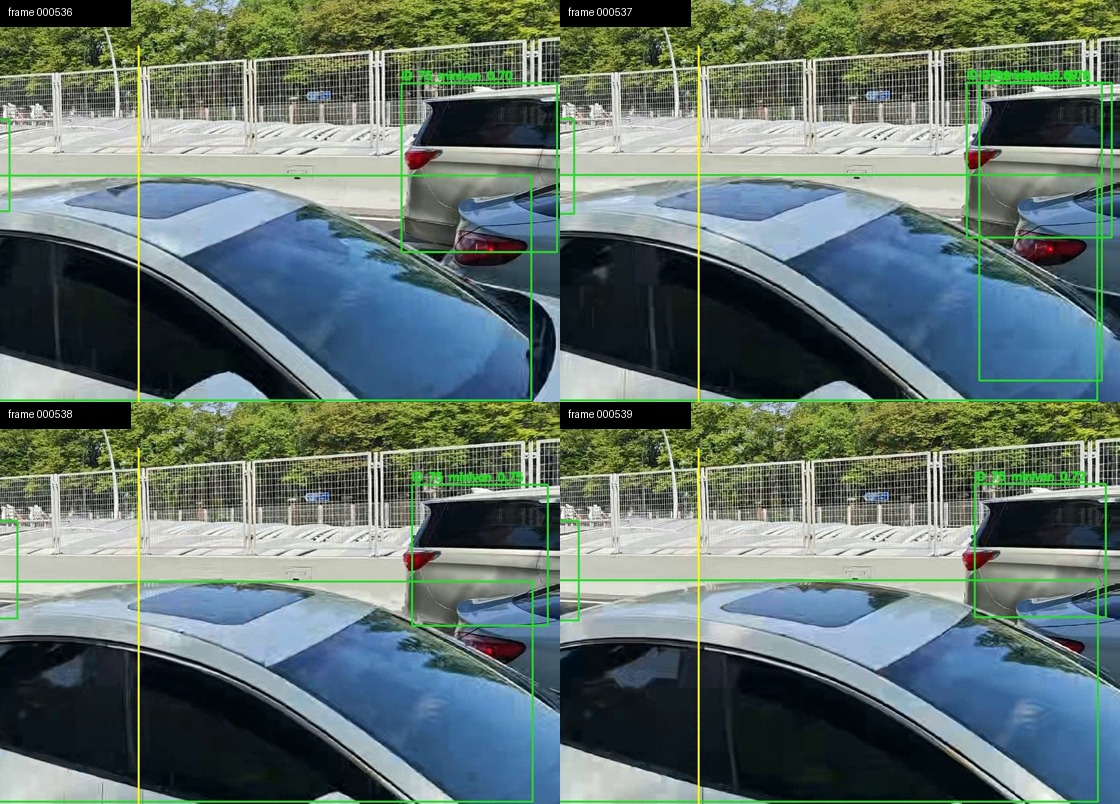
\includegraphics[width=0.92\textwidth]{occlusion_contact_sheet.jpg}
\caption{遮挡片段连续帧}
\end{figure}

该片段中 ID 能够保持的原因可能是目标仍有一部分可见，检测框变化较平滑，ByteTrack 可以利用连续运动和检测置信度完成关联。潜在失败情况包括：遮挡更严重导致检测置信度低于阈值，多个车辆框高度重叠导致 IoU 匹配歧义，或者低帧率和运动模糊使运动预测不稳定。

\section{任务三：U-Net 语义分割}

\subsection{模型与损失函数}

本任务从零实现经典 U-Net，不使用任何预训练分割模型。网络由编码器、解码器和 skip connection 构成：每个 DoubleConv 模块包含两层 $3 \times 3$ 卷积、BatchNorm 和 ReLU；下采样使用 MaxPool；上采样使用 ConvTranspose2d；最后使用 $1 \times 1$ 卷积输出每个像素的类别 logits。

Dice Loss 手动实现为多类别 soft Dice：

\begin{equation}
\mathcal{L}_{Dice}
= 1 - \frac{1}{C}\sum_{c=1}^{C}
\frac{2\sum_i p_{i,c} y_{i,c} + s}
{\sum_i p_{i,c} + \sum_i y_{i,c} + s + \epsilon},
\end{equation}

其中 $p_{i,c}$ 是 softmax 后像素 $i$ 属于类别 $c$ 的概率，$y_{i,c}$ 是 one-hot 标签，$s$ 为平滑项。组合损失为：

\begin{equation}
\mathcal{L} = \mathcal{L}_{CE} + \mathcal{L}_{Dice}.
\end{equation}

\subsection{训练设置}

\begin{table}[H]
\centering
\caption{分割任务主要训练设置}
\begin{tabular}{ll}
\toprule
项目 & 设置 \\
\midrule
输入尺寸 & $256 \times 256$ \\
Batch size & 4 \\
Optimizer & AdamW, learning rate $1\times10^{-3}$, weight decay $1\times10^{-4}$ \\
Base channels & 32；增强实验为 64 \\
Epoch & 50；增强实验为 100 \\
Metric & Validation mIoU \\
\bottomrule
\end{tabular}
\end{table}

\subsection{结果}

\begin{table}[H]
\centering
\caption{Stanford Background 分割结果}
\begin{tabular}{lccc}
\toprule
实验 & Epoch & Val Loss & Val mIoU \\
\midrule
U-Net32 + CE & 50 & 0.5997 & 0.5776 \\
U-Net32 + Dice & 50 & 0.3818 & 0.5566 \\
U-Net32 + CE + Dice & 50 & 1.0844 & \metric{0.6006} \\
U-Net64 + CE + Dice & 100 & 1.1101 & 0.5874 \\
\bottomrule
\end{tabular}
\end{table}

\begin{figure}[H]
\centering
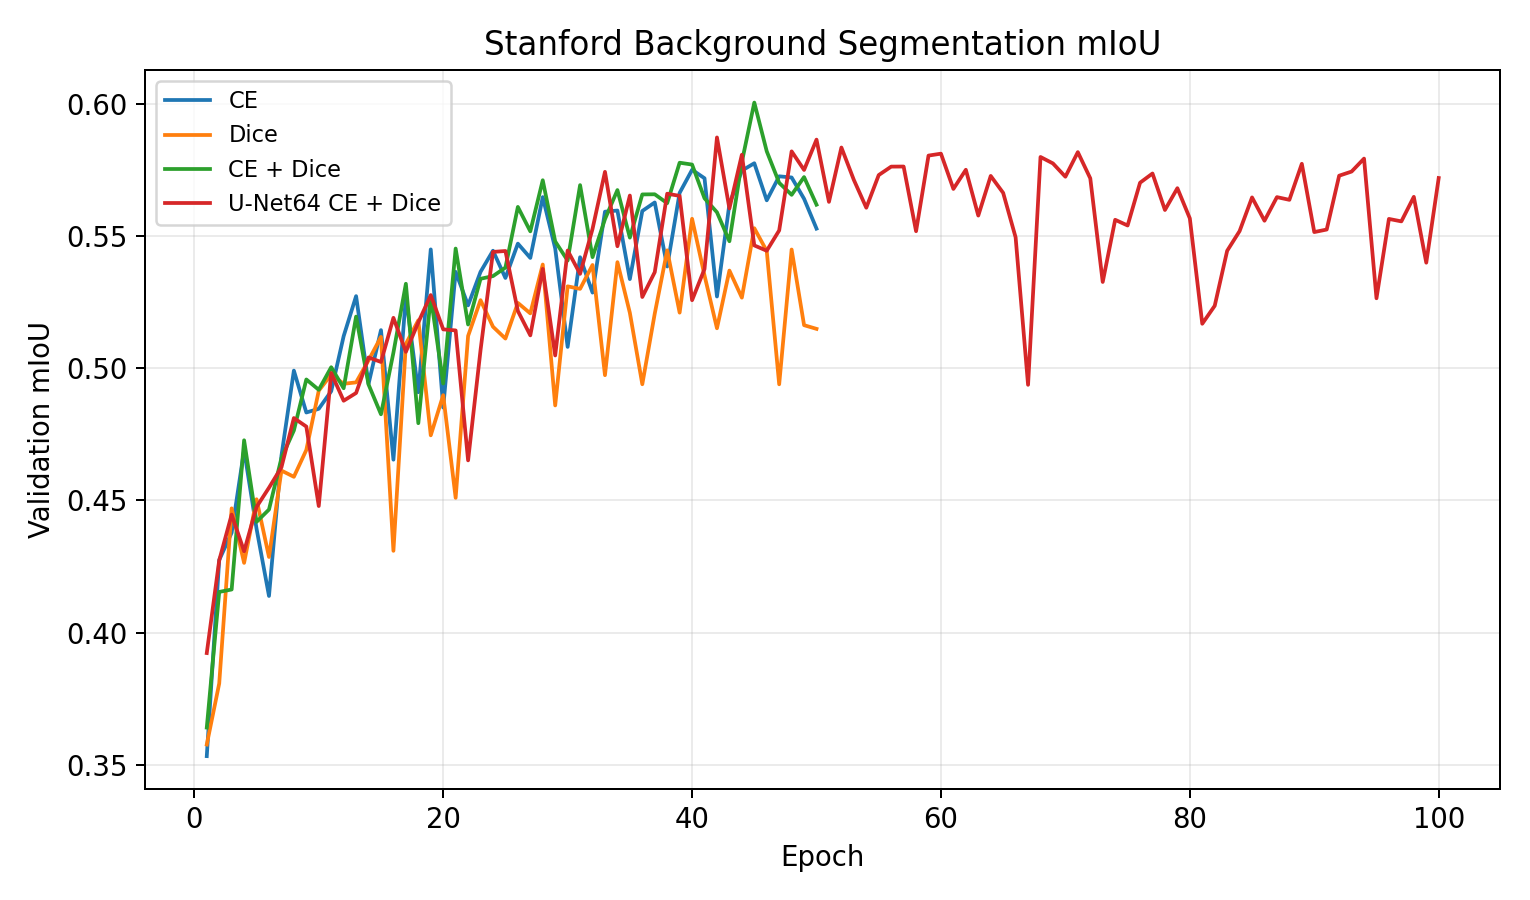
\includegraphics[width=0.82\textwidth]{segmentation_val_miou.png}
\caption{分割任务验证集 mIoU 曲线}
\end{figure}

\begin{figure}[H]
\centering
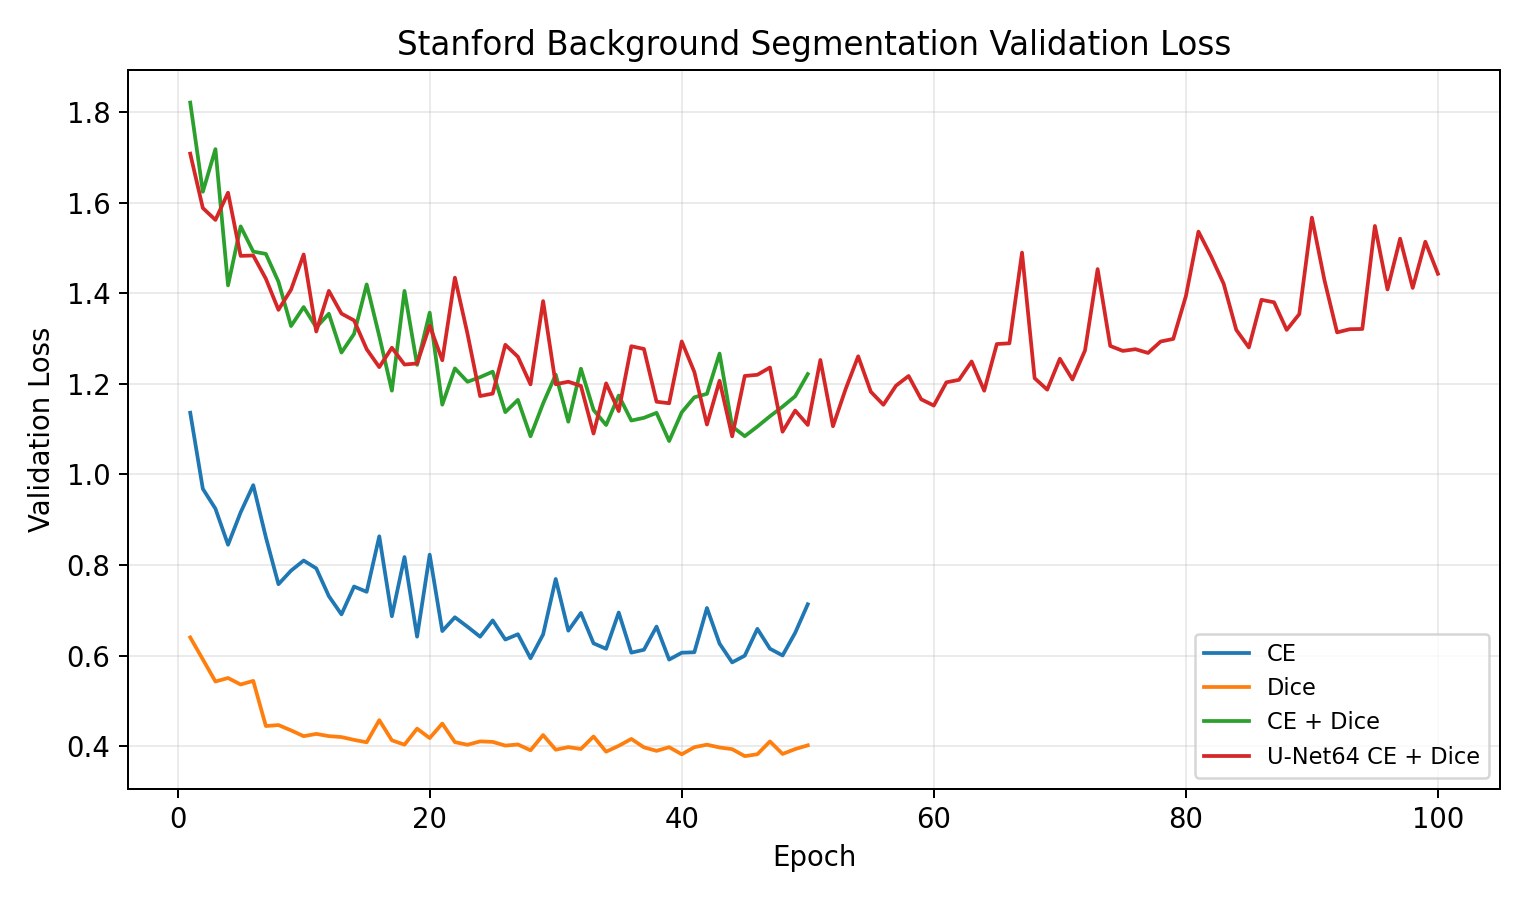
\includegraphics[width=0.82\textwidth]{segmentation_val_loss.png}
\caption{分割任务验证集 Loss 曲线}
\end{figure}

CE + Dice 获得最高验证 mIoU，说明 Dice Loss 对类别面积不均衡有帮助，而 CE Loss 能提供更稳定的逐像素分类监督。Dice 单独训练时 mIoU 低于组合损失，可能是因为 Dice 直接优化区域重叠，对局部像素分类边界的监督不如 CE 稳定。U-Net64 训练 100 epoch 后没有超过 U-Net32 CE + Dice，说明在当前数据规模和设置下，简单增大模型容量不一定带来更好泛化。

\section{结论}

本次作业完成了分类、检测跟踪、语义分割三个任务的完整训练和评估。主要结论如下：

\begin{itemize}
  \item 迁移学习对 Flower102 分类非常关键，预训练 ResNet-18/34 远优于随机初始化。
  \item 车辆检测中 YOLOv8s 明显优于 YOLOv8n，并能支持后续 ByteTrack 视频跟踪、遮挡片段分析和越线计数。
  \item 语义分割中 CE + Dice 是三种损失里效果最好的设置，验证 mIoU 达到 0.6006。
\end{itemize}

后续如果继续改进，可以对 Flower102 尝试更系统的数据增强和学习率调度；对车辆检测增加更多训练轮数或清洗类别标注；对分割任务尝试 class-balanced loss、更多尺度增强或早停策略。

\appendix
\section{复现实验命令}

以下命令均在项目根目录执行，并默认使用 conda 环境 \path{dl_hw2}。

\begin{verbatim}
conda activate dl_hw2

# 第一轮正式训练队列
bash scripts/run_formal_training_queue.sh

# 增强实验队列
bash scripts/run_enhanced_training_queue.sh

# 如果增强训练中断，可从 checkpoint 继续
bash scripts/run_enhanced_training_resume.sh

# 只运行剩余 YOLOv8s 训练/评估
bash scripts/run_enhanced_yolov8s_remaining.sh

# 生成报告图表素材
python scripts/generate_report_assets.py
\end{verbatim}

\section{待提交前补充项}

\begin{enumerate}
  \item 将 GitHub 仓库设为 public，并把链接填入首页。
  \item 将模型权重上传到网盘，并把链接填入首页。
  \item 补全小组成员姓名、学号和具体分工。
  \item 如果老师要求平台截图而不是导出的曲线图，可同步 \path{swanlog/} 后替换或补充 SwanLab 云端截图。
\end{enumerate}

\end{document}
